% =============================================================================
% Template baseado no padrao IComp/UFAM (abntex2)
% Ref: overleaf.com/latex/templates/template-latex-icomp-ufam/ctfssrjvtnjz
% Atividade: Medicao e Analise de RSSI (Wi-Fi) com ESP32 e modelo log-distance
% =============================================================================
\documentclass[
  12pt,
  a4paper,
  oneside,
  brazil,
  chapter=TITLE,
  section=TITLE,
]{abntex2}

% -- Pacotes ------------------------------------------------------------------
\usepackage[T1]{fontenc}
\usepackage[utf8]{inputenc}
\usepackage[brazil]{babel}
\usepackage{times}
\usepackage{microtype}
\usepackage{amsmath,amssymb}
\usepackage{graphicx}
\usepackage{xcolor}
\usepackage{booktabs}
\usepackage{caption}
\usepackage{subcaption}
\usepackage{listings}
\usepackage{float}
\usepackage{enumitem}
\usepackage{indentfirst}
\usepackage{siunitx}
\usepackage{abntex2cite}
\usepackage{hyperref}

\definecolor{ufamblue}{RGB}{0,51,102}
\definecolor{codegreen}{rgb}{0,0.45,0}
\definecolor{codegray}{rgb}{0.5,0.5,0.5}
\definecolor{codeblue}{rgb}{0.1,0.1,0.65}
\definecolor{backcolour}{rgb}{0.97,0.97,0.97}

\lstdefinestyle{cpp}{
  language=C++,
  backgroundcolor=\color{backcolour},
  commentstyle=\color{codegreen}\itshape,
  keywordstyle=\color{codeblue}\bfseries,
  numberstyle=\tiny\color{codegray},
  stringstyle=\color{orange!80!black},
  basicstyle=\ttfamily\scriptsize,
  breaklines=true, keepspaces=true,
  numbers=left, numbersep=6pt,
  frame=single, framerule=0.4pt,
  rulecolor=\color{gray!50}, tabsize=2,
}
\lstdefinestyle{python}{
  language=Python,
  backgroundcolor=\color{backcolour},
  commentstyle=\color{codegreen}\itshape,
  keywordstyle=\color{codeblue}\bfseries,
  numberstyle=\tiny\color{codegray},
  stringstyle=\color{orange!80!black},
  basicstyle=\ttfamily\scriptsize,
  breaklines=true, keepspaces=true,
  numbers=left, numbersep=6pt,
  frame=single, framerule=0.4pt,
  rulecolor=\color{gray!50}, tabsize=4,
}

\hypersetup{
  colorlinks=true,
  linkcolor=ufamblue,
  urlcolor=ufamblue,
  citecolor=ufamblue,
  pdftitle={Medicao e Analise de RSSI Wi-Fi com ESP32 e Modelo Log-Distance},
  pdfauthor={Alison de Oliveira Venancio; Ayrton Finicelli Lemes; Matheus Serrao Uchoa; Victor Ronald},
}

% -- Metadados abntex2 --------------------------------------------------------
\titulo{Medi\c{c}\~ao e An\'alise de RSSI em Redes Wi-Fi:\\
Compara\c{c}\~ao entre Medidas Reais (ESP32) e o Modelo de Propaga\c{c}\~ao Log-Distance}
\autor{Grupo}
\local{Manaus -- AM}
\data{\the\year}
\orientador{Prof. Celso Barbosa Carvalho}
\instituicao{%
  Universidade Federal do Amazonas -- UFAM\\
  Instituto de Computa\c{c}\~ao\\
  Programa de P\'os-Gradua\c{c}\~ao em Engenharia da Computa\c{c}\~ao
}
\tipotrabalho{Relat\'orio T\'ecnico}

\preambulo{Relat\'orio t\'ecnico apresentado \`a disciplina de Redes Sem Fio do
Programa de P\'os-Gradua\c{c}\~ao em Engenharia da Computa\c{c}\~ao da
Universidade Federal do Amazonas (UFAM), como requisito parcial de avalia\c{c}\~ao.}

% Lista de integrantes (capa / folha de rosto)
\newcommand{\integrantes}{%
  \'Alison de Oliveira Ven\^ancio \\[2pt]
  Ayrton Finicelli Lemes \\[2pt]
  Matheus Serr\~ao Uch\^oa \\[2pt]
  Victor Ronald
}

% =============================================================================
\begin{document}
% =============================================================================

\frenchspacing

% -- CAPA (abntex2) -----------------------------------------------------------
\begin{capa}
  \center
  
\includegraphics[width=3.8cm]{../mestrado_ppgee/ufam_logo.png}\\[6pt]
  {\large\bfseries\MakeUppercase{Universidade Federal do Amazonas}}\\[2pt]
  {\normalsize Instituto de Computa\c{c}\~ao}\\[2pt]
  {\normalsize Programa de P\'os-Gradua\c{c}\~ao em Engenharia da Computa\c{c}\~ao}\\[2pt]
  {\normalsize Disciplina: Redes Sem Fio}\\[40pt]

  {\ABNTEXchapterfont\large\MakeUppercase{\imprimirtitulo}}

  \vfill

  {\large\integrantes}

  \vfill

  {\normalsize\imprimirlocal}\\
  {\normalsize\imprimirdata}
\end{capa}

% -- FOLHA DE ROSTO (abntex2) -------------------------------------------------
\begin{folhaderosto}
  \begin{center}
    {\large\bfseries\integrantes}\\[40pt]
    {\ABNTEXchapterfont\large\MakeUppercase{\imprimirtitulo}}\\[40pt]
  \end{center}

  \hspace{.45\textwidth}
  \begin{minipage}{.5\textwidth}
    \imprimirpreambulo\\[8pt]
    \textbf{Professor:} \imprimirorientador
  \end{minipage}

  \vfill
  \begin{center}
    {\normalsize\imprimirlocal}\\
    {\normalsize\imprimirdata}
  \end{center}
\end{folhaderosto}

% -- RESUMO -------------------------------------------------------------------
\begin{resumo}
Este relat\'orio descreve uma atividade pr\'atica de medi\c{c}\~ao e an\'alise
do RSSI (\textit{Received Signal Strength Indicator}) de uma rede Wi-Fi em
ambiente residencial real, comparando os dados coletados com o modelo te\'orico
de propaga\c{c}\~ao \textit{log-distance}. Utilizou-se a plataforma ESP32 para
coletar 30 amostras de RSSI em cada uma de nove dist\^ancias do ponto de acesso
(de \SI{1.0}{\meter} a \SI{5.0}{\meter}, em passos de \SI{0.5}{\meter}),
totalizando 270 medi\c{c}\~oes. Os dados foram organizados em arquivo CSV por um
\textit{script} Python e processados para o c\'alculo das m\'edias por
dist\^ancia. Em paralelo, implementou-se o modelo log-distance parametrizado com
pot\^encia de transmiss\~ao do AP $P_t = \SI{20}{dBm}$, expoente de perda
$n = 3{,}0$ e desvio-padr\~ao de \textit{shadowing} $\sigma = \SI{4}{dB}$,
gerando 30 amostras simuladas por dist\^ancia. A compara\c{c}\~ao mostrou boa
ader\^encia entre teoria e pr\'atica (RMSE de \SI{1.89}{dB} entre as m\'edias),
com expoente de perda efetivo de $n_{ef} = 3{,}23$ estimado por regress\~ao
sobre os dados reais. As discrep\^ancias observadas s\~ao explicadas por
multipercurso, obstru\c{c}\~oes e ru\'ido, refor\c{c}ando a import\^ancia do
termo estoc\'astico de \textit{shadowing} para representar cen\'arios reais.

\vspace{\onelineskip}
\noindent\textbf{Palavras-chave:} RSSI. Wi-Fi. ESP32. Modelo Log-Distance.
Propaga\c{c}\~ao. \textit{Shadowing}. IEEE 802.11.
\end{resumo}

% -- SUMARIO ------------------------------------------------------------------
\pdfbookmark[0]{\contentsname}{toc}
\tableofcontents*
\cleardoublepage

% =============================================================================
\textual
% =============================================================================

% -- 1. INTRODUCAO ------------------------------------------------------------
\chapter{Introdu\c{c}\~ao}

O monitoramento da intensidade do sinal recebido --- expressa pelo RSSI
(\textit{Received Signal Strength Indicator}) --- \'e um dos par\^ametros mais
relevantes em redes sem fio IEEE\,802.11 (Wi-Fi). Al\'em de indicar a qualidade
do enlace, o RSSI fundamenta aplica\c{c}\~oes de localiza\c{c}\~ao
\textit{indoor}, planejamento de cobertura, \textit{handover} e detec\c{c}\~ao
de interfer\^encias \cite{bahl2000radar}.

A rela\c{c}\~ao entre a pot\^encia recebida e a dist\^ancia ao transmissor \'e
descrita por modelos de propaga\c{c}\~ao. O mais difundido em ambientes internos
\'e o modelo \textit{log-distance}, que combina um decaimento determin\'istico
proporcional ao logaritmo da dist\^ancia com um termo estoc\'astico de
\textit{shadowing} (sombreamento) \cite{rappaport2002,goldsmith2005}. Entretanto,
ambientes reais introduzem obst\'aculos, reflex\~oes e m\'ultiplos caminhos que
afastam as medidas das previs\~oes te\'oricas.

Esta atividade tem por objetivo coletar amostras reais de RSSI com a plataforma
ESP32 em fun\c{c}\~ao da dist\^ancia a um ponto de acesso (AP) e compar\'a-las
com o modelo log-distance, discutindo as diferen\c{c}as entre teoria e pr\'atica
e a import\^ancia da modelagem estat\'istica.

% -- 2. OBJETIVOS -------------------------------------------------------------
\chapter{Objetivos}

\section{Objetivo Geral}

Medir o RSSI de uma rede Wi-Fi em fun\c{c}\~ao da dist\^ancia ao ponto de acesso,
em ambiente residencial real, e comparar os resultados com o modelo te\'orico de
propaga\c{c}\~ao \textit{log-distance}.

\section{Objetivos Espec\'ificos}

\begin{enumerate}[label=\alph*)]
  \item Implementar \textit{firmware} ESP32 para enviar leituras de RSSI do AP
        conectado via porta serial;
  \item Coletar 30 amostras de RSSI por dist\^ancia, iniciando a
        $\approx \SI{1}{\meter}$ e afastando-se em passos de \SI{0.5}{\meter}
        at\'e, no m\'inimo, \SI{3}{\meter};
  \item Organizar as leituras em arquivo CSV e calcular a m\'edia por
        dist\^ancia;
  \item Gerar gr\'afico dos dados reais (dist\^ancia $\times$ RSSI m\'edio);
  \item Implementar o modelo log-distance com par\^ametros realistas e gerar
        30 amostras simuladas por dist\^ancia;
  \item Comparar, em um \'unico gr\'afico, os dados reais com a curva te\'orica e
        discutir as discrep\^ancias.
\end{enumerate}

% -- 3. FUNDAMENTACAO TEORICA -------------------------------------------------
\chapter{Fundamenta\c{c}\~ao Te\'orica}

\section{RSSI e Qualidade do Sinal Wi-Fi}

O RSSI mede a pot\^encia do sinal recebido, expressa em dBm (decib\'eis
referidos a \SI{1}{\milli\watt}). Valores t\'ipicos e a respectiva qualidade
percebida s\~ao apresentados na Tabela~\ref{tab:rssi_qualidade}.

\begin{table}[ht]
  \centering
  \caption{Faixas de RSSI e qualidade do sinal Wi-Fi.}
  \label{tab:rssi_qualidade}
  \begin{tabular}{cll}
    \toprule
    \textbf{RSSI (dBm)} & \textbf{Qualidade} & \textbf{Descri\c{c}\~ao} \\
    \midrule
    $> -50$         & Excelente    & Sinal muito forte \\
    $-50$ a $-60$   & Muito bom    & Adequado para \textit{streaming} HD \\
    $-60$ a $-70$   & Bom          & Navega\c{c}\~ao satisfat\'oria \\
    $-70$ a $-80$   & Razo\'avel    & Desempenho reduzido \\
    $-80$ a $-90$   & Fraco        & Instabilidade frequente \\
    $< -90$         & Inutiliz\'avel & Conex\~ao n\~ao confi\'avel \\
    \bottomrule
  \end{tabular}
  \fonte{Adaptado de \citeonline{rappaport2002}.}
\end{table}

\section{Modelo de Propaga\c{c}\~ao Log-Distance}

A perda de percurso (\textit{path loss}) m\'edia cresce logaritmicamente com a
dist\^ancia. O modelo \textit{log-distance} \'e dado pela
Equa\c{c}\~ao~\ref{eq:pathloss} \cite{rappaport2002,goldsmith2005}:

\begin{equation}
  PL(d) = PL(d_0) + 10\,n\log_{10}\!\left(\frac{d}{d_0}\right) + X_\sigma
  \label{eq:pathloss}
\end{equation}

\noindent onde $PL(d)$ \'e a perda \`a dist\^ancia $d$; $PL(d_0)$ \'e a perda na
dist\^ancia de refer\^encia $d_0$ (tipicamente \SI{1}{\meter}); $n$ \'e o
expoente de perda de percurso; e $X_\sigma \sim \mathcal{N}(0,\sigma^2)$ \'e o
termo gaussiano de \textit{shadowing}, em dB.

A pot\^encia recebida (RSSI) relaciona-se com a pot\^encia transmitida $P_t$
pela Equa\c{c}\~ao~\ref{eq:rssi}:

\begin{equation}
  RSSI(d) = P_t - PL(d) = \underbrace{\big[P_t - PL(d_0)\big]}_{RSSI(d_0)}
            - 10\,n\log_{10}\!\left(\frac{d}{d_0}\right) + X_\sigma
  \label{eq:rssi}
\end{equation}

O expoente $n$ depende do ambiente: $n = 2$ no espa\c{c}o livre e tipicamente
$n = 2{,}7$ a $4{,}3$ em ambientes internos com paredes e mobili\'ario
\cite{rappaport2002}. O desvio-padr\~ao do \textit{shadowing} situa-se, em geral,
entre \SI{3}{dB} e \SI{12}{dB}, conforme o grau de obstru\c{c}\~ao
\cite{goldsmith2005,molisch2011}.

\section{Multipercurso e Sombreamento}

Em ambientes fechados, o sinal alcan\c{c}a o receptor por m\'ultiplos caminhos
(reflex\~oes em paredes, piso, teto e mobili\'ario). A soma vetorial dessas
componentes pode ser construtiva ou destrutiva, gerando flutua\c{c}\~oes de
pequena escala (\textit{fading}) sobrepostas \`a tend\^encia de grande escala
descrita pelo termo $X_\sigma$ \cite{molisch2011}. Por isso, medidas reais
raramente decaem de forma estritamente mon\'otona com a dist\^ancia.

\section{Plataforma ESP32}

O ESP32-WROOM-32, da Espressif Systems, integra em um \textit{System-on-Chip}
um processador \textit{dual-core} Xtensa LX6 a \SI{240}{\mega\hertz} com Wi-Fi
802.11\,b/g/n (\SI{2.4}{\giga\hertz}) \cite{esp32datasheet2023}. A API
\texttt{WiFi.RSSI()} retorna o RSSI, em dBm, do AP atualmente conectado
\cite{espressifwifi2023}, o que o torna adequado para campanhas de medi\c{c}\~ao
de baixo custo.

% -- 4. MATERIAIS E METODOLOGIA -----------------------------------------------
\chapter{Materiais e Metodologia}

\section{Materiais}

\begin{itemize}
  \item \textbf{Hardware:} placa ESP32-WROOM-32 \textit{Dev Module};
  \item \textbf{Ponto de acesso:} roteador residencial \SI{2.4}{\giga\hertz},
        pot\^encia de transmiss\~ao $P_t \approx \SI{20}{dBm}$
        (\SI{100}{\milli\watt} EIRP), dentro do limite de radia\c{c}\~ao
        restrita da ANATEL \cite{anatel2017};
  \item \textbf{IDE:} Arduino IDE 2.x com suporte ESP32 (Espressif 3.x);
  \item \textbf{Linguagens:} C++ (Arduino) e Python 3.11;
  \item \textbf{Bibliotecas Python:} \texttt{pyserial}, \texttt{numpy},
        \texttt{matplotlib}.
\end{itemize}

\section{Local da Coleta}

A campanha foi realizada em uma resid\^encia localizada na Travessa Castelo
Branco, bairro Compensa, Manaus/AM. As medi\c{c}\~oes ocorreram ao longo de um
corredor interno conectado \`a sala, com paredes de alvenaria e mobili\'ario
t\'ipico, condi\c{c}\~ao representativa de um ambiente residencial urbano
amaz\^onico densamente ocupado por redes Wi-Fi vizinhas na faixa de
\SI{2.4}{\giga\hertz}.

\section{Procedimento}

\begin{enumerate}
  \item Carga do \textit{firmware} \texttt{envia\_rssi.ino} no ESP32, conectando
        ao AP sob medi\c{c}\~ao;
  \item Posicionamento do ESP32 a \SI{1.0}{\meter} do AP e coleta de 30 amostras
        de RSSI com o \textit{script} \texttt{coleta\_dados.py};
  \item Afastamento em passos de \SI{0.5}{\meter} (\num{1.0}, \num{1.5},
        \ldots, \SI{5.0}{\meter}), repetindo a coleta de 30 amostras em cada
        ponto --- totalizando 9 dist\^ancias e 270 medi\c{c}\~oes;
  \item C\'alculo da m\'edia e do desvio-padr\~ao por dist\^ancia
        (\texttt{grafico\_valor\_medio.py});
  \item Simula\c{c}\~ao do modelo log-distance (\texttt{log\_distancia.py}) com
        $P_t = \SI{20}{dBm}$, $n = 3{,}0$ e $\sigma = \SI{4}{dB}$;
  \item Compara\c{c}\~ao entre dados reais e curva te\'orica
        (\texttt{grafico\_comparativo.py}).
\end{enumerate}

% -- 5. IMPLEMENTACAO ---------------------------------------------------------
\chapter{Implementa\c{c}\~ao}

\section{Firmware ESP32 (\texttt{envia\_rssi.ino})}

O \textit{firmware} conecta o ESP32 ao AP e envia o RSSI do enlace pela serial a
cada \SI{200}{\milli\second}, uma leitura por linha.

\lstinputlisting[style=cpp,
  caption={Firmware ESP32 --- envio peri\'odico do RSSI do AP conectado.},
  label={lst:firmware}]{envia_rssi.ino}

\section{Coleta Serial (\texttt{coleta\_dados.py})}

O \textit{script} l\^e a serial, agrupa 30 amostras por dist\^ancia informada
pelo operador e grava em \texttt{medicoes\_rssi.csv}.

\lstinputlisting[style=python,
  caption={Coleta e organiza\c{c}\~ao das amostras de RSSI por dist\^ancia.},
  label={lst:coleta}]{coleta_dados.py}

\section{Modelo Log-Distance (\texttt{log\_distancia.py})}

Implementa a Equa\c{c}\~ao~\ref{eq:rssi}, gerando 30 amostras simuladas de RSSI
por dist\^ancia e a respectiva m\'edia.

\lstinputlisting[style=python,
  caption={Simula\c{c}\~ao do modelo log-distance (30 amostras por dist\^ancia).},
  label={lst:logdist}]{log_distancia.py}

\section{Gr\'afico Comparativo (\texttt{grafico\_comparativo.py})}

Sobrep\~oe os dados reais \`a curva te\'orica, ajusta o expoente $n$ efetivo dos
dados reais e quantifica a ader\^encia (RMSE e MAE).

\lstinputlisting[style=python,
  caption={Compara\c{c}\~ao entre dados reais e modelo log-distance.},
  label={lst:comp}]{grafico_comparativo.py}

% -- 6. RESULTADOS ------------------------------------------------------------
\chapter{Resultados}

\section{Parte 1 --- Dados Coletados}

Foram coletadas 270 amostras (9 dist\^ancias $\times$ 30 amostras). A
Tabela~\ref{tab:medias} resume a m\'edia, o desvio-padr\~ao e os extremos do
RSSI por dist\^ancia; um excerto das amostras brutas \'e mostrado na
Tabela~\ref{tab:excerto}. O conjunto completo encontra-se em
\texttt{medicoes\_rssi.csv}.

\begin{table}[H]
  \centering
  \caption{RSSI por dist\^ancia --- m\'edia, desvio-padr\~ao e extremos (30 amostras).}
  \label{tab:medias}
  \begin{tabular}{cccccc}
    \toprule
    \textbf{Dist. (m)} & \textbf{M\'edia (dBm)} & \textbf{Desvio (dB)} &
    \textbf{M\'in (dBm)} & \textbf{M\'ax (dBm)} & \textbf{$n$} \\
    \midrule
    1{,}0 & $-40{,}03$ & 1{,}33 & $-42$ & $-37$ & 30 \\
    1{,}5 & $-45{,}00$ & 1{,}66 & $-49$ & $-42$ & 30 \\
    2{,}0 & $-49{,}30$ & 2{,}09 & $-54$ & $-46$ & 30 \\
    2{,}5 & $-50{,}23$ & 2{,}01 & $-54$ & $-47$ & 30 \\
    3{,}0 & $-55{,}37$ & 2{,}09 & $-59$ & $-52$ & 30 \\
    3{,}5 & $-57{,}23$ & 1{,}91 & $-62$ & $-53$ & 30 \\
    4{,}0 & $-60{,}80$ & 3{,}11 & $-68$ & $-56$ & 30 \\
    4{,}5 & $-59{,}13$ & 2{,}70 & $-65$ & $-53$ & 30 \\
    5{,}0 & $-62{,}50$ & 3{,}36 & $-70$ & $-58$ & 30 \\
    \bottomrule
  \end{tabular}
  \fonte{Elaborado pelos autores (2026).}
\end{table}

\begin{table}[H]
  \centering
  \caption{Excerto do arquivo \texttt{medicoes\_rssi.csv} (amostras a \SI{1.0}{\meter}).}
  \label{tab:excerto}
  \small
  \begin{tabular}{ccc}
    \toprule
    \textbf{distancia\_m} & \textbf{amostra} & \textbf{rssi\_dbm} \\
    \midrule
    1.0 & 1 & $-39$ \\
    1.0 & 2 & $-42$ \\
    1.0 & 3 & $-41$ \\
    1.0 & 4 & $-39$ \\
    1.0 & 5 & $-40$ \\
    \multicolumn{3}{c}{\ldots} \\
    \bottomrule
  \end{tabular}
  \fonte{Elaborado pelos autores (2026).}
\end{table}

\section{Parte 2 --- Gr\'afico dos Dados Reais}

A Figura~\ref{fig:real} apresenta o RSSI m\'edio em fun\c{c}\~ao da dist\^ancia,
com barras de desvio-padr\~ao. Observa-se o decaimento esperado, com pequenas
inflex\~oes em \SI{2.5}{\meter} e \SI{4.5}{\meter}.

\begin{figure}[H]
  \centering
  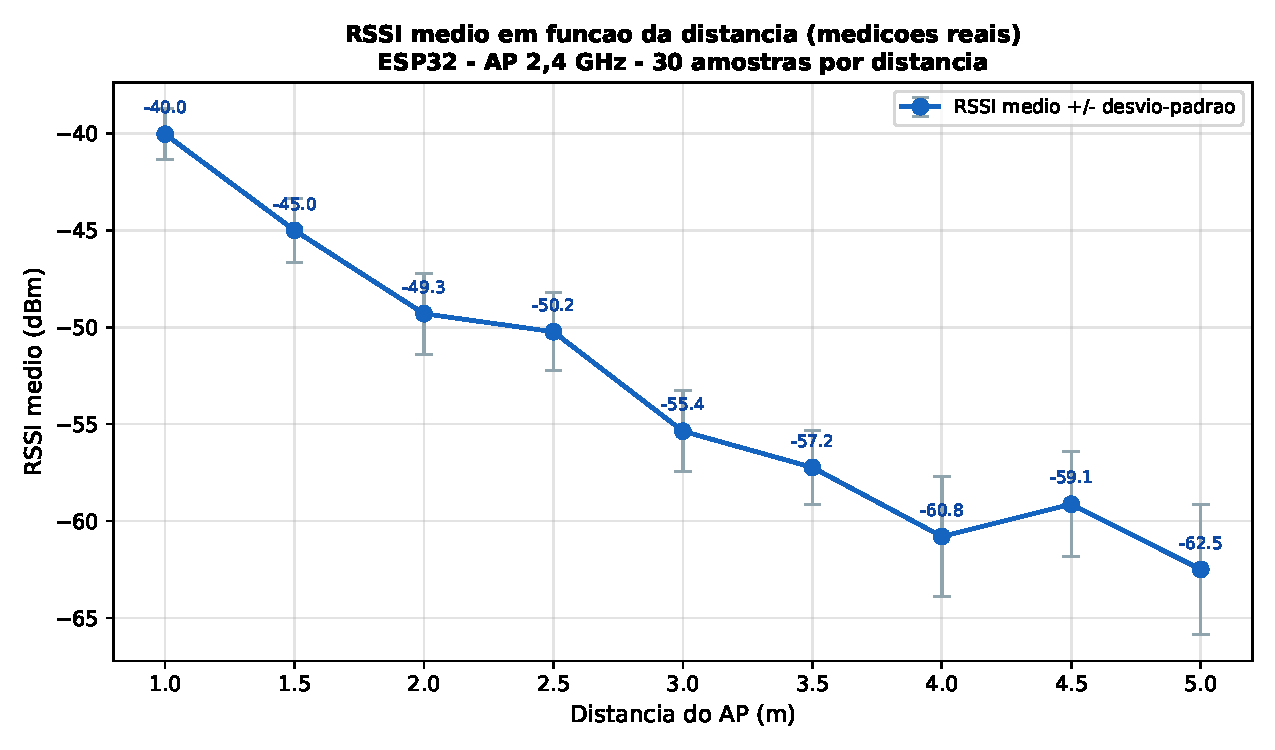
\includegraphics[width=0.92\linewidth]{images/rssi_medio_real.pdf}
  \caption{RSSI m\'edio medido em fun\c{c}\~ao da dist\^ancia ao AP
           (30 amostras por dist\^ancia).}
  \label{fig:real}
  \fonte{Elaborado pelos autores (2026).}
\end{figure}

\section{Parte 3 --- Simula\c{c}\~ao Te\'orica}

A Figura~\ref{fig:teorico} mostra as 30 amostras simuladas por dist\^ancia, a
m\'edia simulada e a curva te\'orica sem ru\'ido, obtidas com $P_t = \SI{20}{dBm}$,
$n = 3{,}0$ e $\sigma = \SI{4}{dB}$.

\begin{figure}[H]
  \centering
  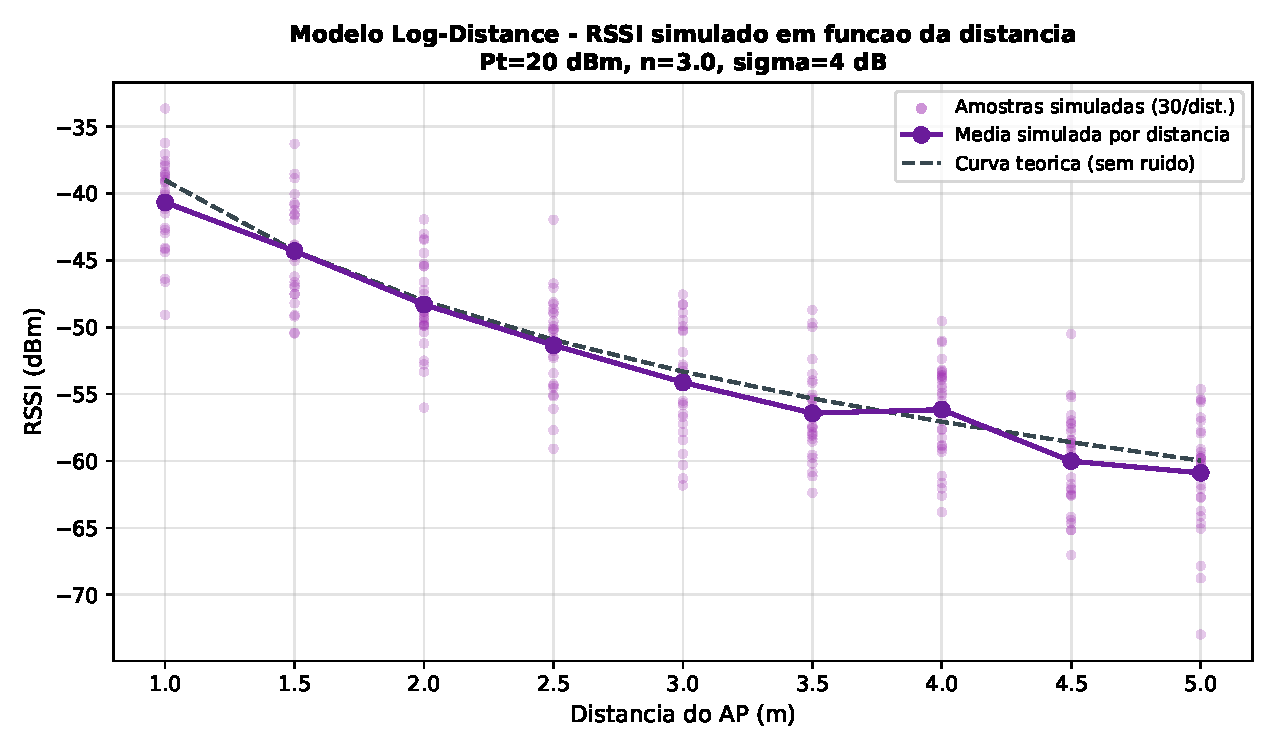
\includegraphics[width=0.92\linewidth]{images/rssi_medio_teorico.pdf}
  \caption{RSSI simulado pelo modelo log-distance: amostras, m\'edia e curva
           te\'orica.}
  \label{fig:teorico}
  \fonte{Elaborado pelos autores (2026).}
\end{figure}

\section{Parte 4 --- Gr\'afico Comparativo}

A Figura~\ref{fig:comp} sobrep\~oe os dados reais \`a curva te\'orica e \`a faixa
de incerteza $\pm\sigma$. Todos os pontos reais permanecem dentro da faixa
te\'orica. O ajuste por regress\~ao sobre os dados reais forneceu expoente
efetivo $n_{ef} = 3{,}23$ (\textit{vs.} $n = 3{,}0$ te\'orico), com
RMSE de \SI{1.89}{dB} e MAE de \SI{1.61}{dB} entre as m\'edias.

\begin{figure}[H]
  \centering
  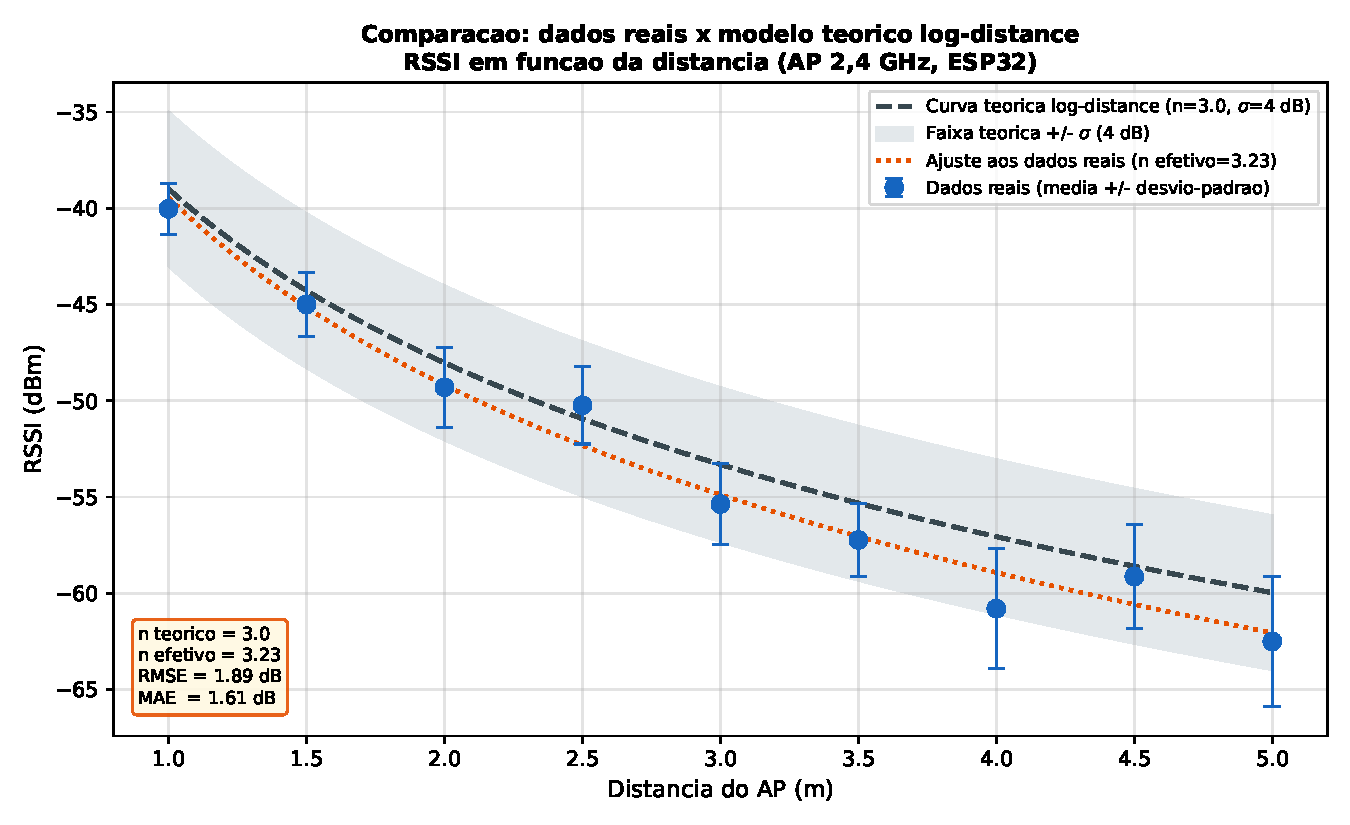
\includegraphics[width=\linewidth]{images/comparativo.pdf}
  \caption{Compara\c{c}\~ao entre os dados reais (pontos) e o modelo te\'orico
           log-distance (linha tracejada) com faixa $\pm\sigma$.}
  \label{fig:comp}
  \fonte{Elaborado pelos autores (2026).}
\end{figure}

% -- 7. ANALISE E DISCUSSAO ---------------------------------------------------
\chapter{An\'alise e Discuss\~ao}

\section{Diferen\c{c}as entre Teoria e Pr\'atica}

A ader\^encia global entre as medidas e o modelo foi boa: o RMSE de
\SI{1.89}{dB} \'e da ordem de uma fra\c{c}\~ao do desvio-padr\~ao de
\textit{shadowing} adotado ($\sigma = \SI{4}{dB}$), e todos os pontos reais
ca\'iram dentro da faixa $\pm\sigma$ (Figura~\ref{fig:comp}). Ainda assim, o
expoente de perda efetivo dos dados reais ($n_{ef} = 3{,}23$) foi superior ao
valor te\'orico assumido ($n = 3{,}0$), indicando atenua\c{c}\~ao um pouco mais
acentuada do que a prevista. As medidas mostraram-se sistematicamente
ligeiramente abaixo da curva te\'orica a partir de \SI{3.0}{\meter}, e
n\~ao-monot\^onicas em \SI{2.5}{\meter} e \SI{4.5}{\meter}, onde o RSSI medido
superou o do ponto anterior --- comportamento incompat\'ivel com o decaimento
puramente determin\'istico do modelo.

\section{Fatores que Explicam as Discrep\^ancias}

\begin{itemize}
  \item \textbf{Obst\'aculos e obstru\c{c}\~oes:} mobili\'ario e trechos de
        parede no percurso adicionam atenua\c{c}\~ao localizada (por exemplo, a
        queda acentuada em \SI{4.0}{\meter}), elevando o expoente efetivo;
  \item \textbf{Reflex\~oes e multipercurso:} a soma construtiva de componentes
        refletidas explica os ``picos'' de RSSI em \SI{2.5}{\meter} e
        \SI{4.5}{\meter}, em que o sinal medido foi melhor que o do ponto
        anterior;
  \item \textbf{Ru\'ido e interfer\^encia cocanal:} a faixa de
        \SI{2.4}{\giga\hertz} \'e densamente ocupada por redes vizinhas no
        ambiente residencial urbano, aumentando a vari\^ancia das leituras
        (note-se o crescimento do desvio-padr\~ao com a dist\^ancia,
        de \SI{1.33}{dB} a \SI{3.36}{dB});
  \item \textbf{Fatores de \textit{hardware}:} a efici\^encia e o diagrama de
        irradia\c{c}\~ao das antenas do ESP32 e do AP, al\'em da quantiza\c{c}\~ao
        inteira do RSSI, introduzem desvios adicionais;
  \item \textbf{Din\^amica do ambiente:} a movimenta\c{c}\~ao de pessoas durante
        a coleta provoca \textit{shadowing} vari\'avel no tempo.
\end{itemize}

\section{Import\^ancia da Modelagem Estat\'istica}

Os resultados evidenciam que um modelo puramente determin\'istico
(termo $10\,n\log_{10}(d/d_0)$) \'e insuficiente para representar o
comportamento real do canal: sem o termo estoc\'astico $X_\sigma$, n\~ao seria
poss\'ivel explicar nem a dispers\~ao das 30 amostras em cada dist\^ancia nem as
inflex\~oes n\~ao-monot\^onicas observadas. A modelagem estat\'istica do
\textit{shadowing} via vari\'avel gaussiana de desvio $\sigma$ \'e o que permite
delimitar a faixa de incerteza ($\pm\sigma$) na qual as medidas efetivamente
ocorrem. Esse tratamento probabil\'istico \'e essencial para o
dimensionamento de margens de enlace (\textit{link budget}), para o
planejamento de cobertura e, sobretudo, para sistemas de localiza\c{c}\~ao
\textit{indoor} baseados em RSSI, nos quais a incerteza do sinal precisa ser
modelada explicitamente \cite{bahl2000radar,goldsmith2005}.

% -- 8. CONCLUSAO -------------------------------------------------------------
\chapter{Conclus\~ao}

A atividade cumpriu todos os objetivos propostos. Foram coletadas 270 amostras
reais de RSSI com o ESP32 em nove dist\^ancias (de \SI{1.0}{} a \SI{5.0}{\meter}),
organizadas em CSV e reduzidas \`as m\'edias por dist\^ancia. O modelo
log-distance foi implementado com par\^ametros realistas ($P_t = \SI{20}{dBm}$,
$n = 3{,}0$, $\sigma = \SI{4}{dB}$) e comparado aos dados reais em um \'unico
gr\'afico.

A compara\c{c}\~ao revelou boa concord\^ancia (RMSE de \SI{1.89}{dB};
$n_{ef} = 3{,}23$), com discrep\^ancias atribu\'iveis a multipercurso,
obst\'aculos, ru\'ido e caracter\'isticas de \textit{hardware}. Conclui-se que o
modelo log-distance reproduz adequadamente a tend\^encia m\'edia de decaimento,
desde que acompanhado do termo estoc\'astico de \textit{shadowing}, sem o qual
n\~ao se representam as flutua\c{c}\~oes inerentes ao canal real. Como trabalho
futuro, sugere-se estender a campanha a maiores dist\^ancias e a m\'ultiplos
ambientes, bem como aplicar filtragem por m\'edia m\'ovel para mitigar o ru\'ido
de pequena escala.

% =============================================================================
\postextual
% =============================================================================

% -- REFERENCIAS --------------------------------------------------------------
\bibliography{referencias}

\end{document}
